%%%%%%%%%%%%%%%%%%%%%%%%%%%%%%%%%%%%%%%%%%%%%%%%%%%%%%%%%%%%%%%%%
% Lecture date: 19-12-18
%%%%%%%%%%%%%%%%%%%%%%%%%%%%%%%%%%%%%%%%%%%%%%%%%%%%%%%%%%%%%%%%%
\chapter{Non-abelian Gauge Theories}
\section{Reminder: Gauge invariance}
Demand invariance of Dirac theory under \underline{local} phase transformation
\begin{align*}
   \psi (x) \mapsto \euler^{i\alpha(x)}\psi(x).
\end{align*}

To have invariant Lagrangian density, mass term $- m \bar\psi (x) \psi (x)$ causes no problem. Definition of directional derivative by
\begin{align}
   n^\mu \partial_\mu \psi = \lim_{\epsilon \rightarrow 0} \frac{1}{\epsilon} \left[ \psi(x+\epsilon n) + \psi(x) \right].
\end{align}
$\psi(x+\epsilon n )$ and $\psi(x)$ have different behaviour under local phase (gauge) transformation. 

Compensate this by introducing an operator
\begin{align}
   U(y , x) \mapsto \euler^{i\alpha(y)} U(y,x) \euler^{-i\alpha(x)}, \label{math:Utrafo}
\end{align}
with $U(x,x) = 1$ and $U(y,x) = \euler^{i\phi(x,y)}$.

Then define \underline{covariant derivative}
\begin{align}
   n^\mu D_\mu \psi = \lim_{\epsilon \rightarrow 0} \frac{1}{\epsilon} \left[ \psi(x + \epsilon n ) - U(x+\epsilon n, x) \psi(x) \right].
\end{align}
Infinitesimally,
\begin{align}
   U(x+\epsilon n , x) = 1+ ie \epsilon n^\mu A_\mu (x) + \order{\epsilon^2}. \label{math:UInf}
\end{align}
It defines vector field $A_\mu$. The covariant derivative is 
\begin{align}
   D_\mu \psi (x) = \partial_\mu \psi (x) - ie A_\mu (x) \psi (x).
\end{align}

Combine (\ref{math:Utrafo}) and (\ref{math:UInf}), 
\begin{align*}
   1 + i e \epsilon n \cdot A(x) &\rightarrow ( 1 + i\alpha(x + \epsilon n)) (1 + ie \epsilon n \cdot A(x)) (1 - i\alpha(x)), \\
                                 & = 1+ ie \epsilon n \cdot  \left( A(x) + \frac{1}{e} \partial\alpha(x) \right) + \order{\epsilon^2}.
\end{align*}
Hence the vector field transforms according to
\begin{align}
   A_\mu (x) \mapsto A_\mu (x) + \frac{1}{e } \partial_\mu \alpha(x)
\end{align} 

Covariant derivative is indeed covariant
\begin{align*}
   D_\mu \psi(x) &\mapsto \left[ \partial_\mu - ie \left( A_\mu + \frac{1}{e} \partial_\mu \alpha(x) \right) \right] \euler^{i\alpha(x)} \psi(x), \\
                 &= \euler^{i\alpha(x)} \left( \partial_\mu - ie A_\mu \right) \psi (x), \\
                 &= \euler^{i \alpha(x)} D_\mu \psi(x).
\end{align*}
In this way, we can construct derivative terms invariant under local phase transformation $i \bar{\psi} \slashed{D} \psi$ and potentially higher derivative if we don't care about renormalizability.

The field $A_\mu(x)$ also need kinetic term(s). Also second covariant derivatives are covariant, in particular,
\begin{align*}
   \left[ D_\mu, D_\nu \right] \psi &\mapsto \euler^{i \alpha(x)} \left[ D_\mu, D_\nu \right] \psi (x), \\
                                    &= \comm{\partial_\mu, \partial_\nu} \psi - ie \left( \comm{\partial_\mu}{A_\nu} - \comm{\partial_\nu}{A_\mu} \right) \psi - e^2 \comm{A_\mu}{A_\nu} \psi, 
                                    \shortintertext{We are dealing with classical theory at the moment. The commutator of the fields is zero.}
                                    &= -ie \left( \partial_\mu A_\nu - \partial_\nu A_\mu \right) \psi, \\
                                    &= -ie F_{\mu\nu}.
\end{align*}
Conclude $F_{\mu\nu}$ is invariant under local phase transformation.

All operators up to dimension $4$
\begin{align}
   \lag_4 = i \bar{\psi}  \slashed{D} \psi - m \bar{\psi} \psi - \frac{1}{4} F_{\mu\nu} F^{\mu\nu} - e \epsilon_{\mu \nu \alpha \beta} F^{\mu\nu} F^{\alpha \beta}
\end{align}

\section{Yang-Mills Fields}
It is the simplest example for a non-abelian gauge theory and was originally gauge theory for isospin.

Consider $\psi$ with spinor in Minkowski space and "isospinor" in isospin space 
\begin{align}
   \psi (x) = \begin{pmatrix} \psi_1 (x) \\ \psi_2 (x)\end{pmatrix}
\end{align}

Promote standard isospin invariant to a local transformation
\begin{align}
   \psi(x) &\mapsto V(x) \psi(x), \\
   V(x) &= \exp(i\alpha^i(x) \sigma^i / 2),
\end{align}
with $\sigma^i$ Pauli matrices and $V(x) \in \mathbf{SU}(2) $. It is non-abelian, because different elements of $\mathbf{SU}(2)$ in general don't commute.

Repeat the construction from the previous section here. The transformation of an unitary matrix 
\begin{align}
   U(y, x) \mapsto V(y) U(y ,x) V(x)^\dagger,
\end{align}
with $U(x,x) = \id$. It is used for the construction of a covariant derivative. Infinitesimally,
\begin{align}
   U(x+\epsilon n, x) = \id + ig \epsilon n^\mu A_\mu^i \sigma^i /2 + \order{\epsilon^2}.
\end{align}
There are three vector fields $A_\mu^i$ with $i=1,2,3$.

Covariant derivative 
\begin{align}
   D_\mu = \partial_\mu - ig A_\mu^i \sigma^i /2
\end{align}
The transformation of $A_\mu^i$ is
\begin{align*}
   1 + ig \epsilon n^\mu A_\mu^i \sigma^i /2 &\mapsto V(x + \epsilon n) (1 + ig\epsilon n^\mu A_\mu^i \sigma^i /2) V(x)^\dagger. 
   \shortintertext{Expand this to linear order in $\epsilon$,}
   V(x + \epsilon n ) V(x)^\dagger &= \left[ (1+\epsilon n^\mu \partial_\mu) V(x) \right] V(x)^\dagger + \order{\epsilon^2} \\
                                   & = \id + \epsilon n^\mu (\partial_\mu V(x)) V(x)^\dagger + \order{\epsilon^2} \\
                                   &= \id - \epsilon n^\mu V(x) (\partial_\mu V(x)^\dagger) + \order{\epsilon^2}
\end{align*}
Hence
\begin{align}
   \frac{1}{2}A_\mu^i \sigma^i \mapsto V(x) \left[ \frac{1}{2} A_\mu^i \sigma^i + \frac{i}{g} \partial_\mu \right] V(x)^\dagger .
\end{align}

For infinitesimal transformation $V(x) = \id + \frac{i}{2} \alpha^i (x) \sigma^i  + \order{\alpha^2}$. We find
\begin{align}
   \frac{1}{2}A_\mu^i \sigma^i &\mapsto \frac{1}{2} A_\mu^i \sigma^i + \frac{1}{2g} (\partial_\mu \alpha^i) \sigma^i + \frac{i}{4} \alpha^i A_\mu^j \comm{\sigma^i}{\sigma^j}, \\
   A_\mu^i &\mapsto A_\mu^i + \frac{1}{g} \partial_\mu \alpha^i - \epsilon^{ijk} \alpha^j A_\mu^k.
\end{align}
Third terms acts like a gauge field and third like an isovector. The isovector term is  new compared to the abelian theory. Consequence of the non-commuting local transformation.

Introducing notation $\tilde{X} = \frac{1}{2} X^i \sigma^i $. Covariant derivative is now  
\begin{align}
   D_\mu \psi &\mapsto \left( \partial_\mu - ig \tilde{A}_\mu - i \partial_\mu \tilde{\alpha} + g \comm{\tilde{\alpha}}{\tilde A} \right) (1 + i \tilde{\alpha}) \psi(x), \notag \\
              &= \left(\partial_\mu + i \tilde{\alpha}\partial_\mu - ig \tilde{A}_\mu + g \tilde{A}_\mu \tilde{\alpha} + g \comm{\tilde{\alpha}}{\tilde{A}} + \order{\alpha^2}\right) \psi, \notag \\
              &= (1 + i \tilde{\alpha}) (\partial_\mu - ig \tilde{A}_\mu) \psi + \order{\alpha^2}, \notag \\
              &= (1+ i\tilde{\alpha}) D_\mu \psi + \order{\alpha^2}.
\end{align}

Introduce field strength through  commutator of two covariant derivatives
\begin{align}
   \comm{D_\mu}{D_\nu} = -ig \tilde{F}_{\mu\nu},
\end{align}
with
\begin{align}
   \tilde{F}_{\mu\nu} &= \partial_\mu \tilde{A}_\nu - \partial_\nu \tilde{A}_\mu - ig \comm{\tilde{A}_\mu}{\tilde{A}_\nu}, \\
   F_{\mu\nu}^i &= \partial_\mu A_\nu^i - \partial_\nu A_\mu^i + g \epsilon^{ijk} A^j_\mu A^k_\nu.
\end{align} 

Transformation behaviour of $\tilde{F}_{\mu\nu}$ from $\psi \mapsto V\psi$, $\comm{D_\mu}{D_\nu} \psi \mapsto V \comm{D_\mu}{D_\nu} \psi$
\begin{align*}
   \tilde{F}_{\mu\nu}(x) \mapsto V(x) \tilde{F}_{\mu\nu}(x) V(x)^\dagger.
\end{align*}
$\tilde{F}_{\mu\nu}$ is not gauge invariant any more.

Gauge invariant Lagrangian terms are however easily constructed
\begin{align}
   \lag = -\frac{1}{2} \tr (\tilde{F}_{\mu\nu} \tilde{F}^{\mu\nu}) =  -\frac{1}{4} F^i_{\mu\nu} F^{i \; \mu\nu}.
\end{align}
Trace is taken in isospin space: $\tr(\sigma^i \sigma^j) = 2\delta^{ij}$. Note that in contrast to the abelian case, $\tr(\tilde{F}\tilde{F})$ contains cubic and quartic terms in $A_\mu^i$, hence already describes an \underline{interacting} theory, not a free one.

Complete YM Lagrangian density
\begin{align}
   \lag = - \frac{1}{2} \tr (\tilde{F}_{\mu\nu} \tilde{F}^{\mu\nu}) + \bar\psi ( i \slashed{D} - m) \psi.
\end{align}
Field equations are 
\begin{align*}
   (i\slashed{D} - m) \psi  &= 0, \\
   \comm{D^\mu}{\tilde{F}_{\mu\nu}} &= -g \tilde{j}_\nu,
\end{align*}
with $j_\nu^i =\frac{1}{2} \bar\psi \gamma_\nu \sigma^i \psi $. These are highly non-linear set of equations.

Now
\begin{align*}
   \comm{D_\mu}{\comm{D_\nu}{\tilde{F}^{\mu\nu}}} &= \frac{1}{2} \left\{ \comm{D_\mu}{\comm{D_\nu}{\tilde{F}^{\mu\nu}}}  - \comm{D_\nu}{\comm{D_\mu}{\tilde{F}^{\mu\nu}}}\right\} \\
                                                  &= \frac{1}{2} \comm{\comm{D_\mu}{D_nu}}{\tilde{F}^{\mu\nu}}  \\
                                                  &= 0
\end{align*}
Hence, from the second equation of motion
\begin{align}
   \comm{D^\mu}{\tilde{j}_\mu} = \partial^\mu \tilde{j}_\mu - ig \comm{\tilde{A}^\mu}{\tilde{j}_\mu} = 0.
\end{align}
This is the analogue of current conservation in Yang-Mills theory.

All this can be generalized to other (than $\mathbf{SU}(2)$) local symmetry group with 
\begin{align*}
   \sigma^i / 2 \mapsto t^a,
\end{align*}
a new set of hermitian generators and the general \underline{structure constants} $f^{abc}$
\begin{align}
   \comm{t^a}{t^b} = i f^{abc} t^c,
\end{align}
instead of $\epsilon^{ijk}$.

\section{Feynman Rules for Non-abelian Gauge theories}
\begin{align}
   \lag = \bar{\psi} \left( i \slashed{D} - m \right)\psi - \frac{1}{4} F_{\mu\nu}^a F^{a\; \mu\nu}
\end{align}
with 
\begin{align*}
   F^a_{\mu\nu} &= \partial_\mu A_\nu^a - \partial_\nu A^a_\mu + g f^{abc} A_\mu^v A_\nu^c  \\
   D_\mu & = \partial_\mu - igA_\mu^a t^a
\end{align*}

Fermion propagator is as before but with an internal quantum number
\begin{align}
   \braket{0 | T \psi_A (x) \bar{\psi}_B(y) | 0} = \int \frac{\dd[4]{k}}{(2\pi)^4} \frac{i\delta_{AB}}{\slashed{k}-m} \euler^{-ik(x-y)} 
\end{align}
Fermion fields are (in) fundamental representation for $\SU(n)$ with $A,B=1,\dots,n$.

Suspect that there is an analogous gauge field propagator in Feynman gauge 
\begin{align}
   \braket{0 | T A_\mu^a (x) A_\nu^b (y) | 0} = \int \frac{\dd[4]{k}}{(2\pi)^4} \frac{-ig_{\mu\nu} \delta^{ab}}{k^2} \euler^{-ik(x-y)}
\end{align}
Fields $A_\mu(x)$ are in adjoint representation for $\SU(n)$ with $a,b = 1, \dots, n^2 - 1$.

Interaction terms are
\begin{align}
   \lag = \lag_0 + g A_\lambda^a \bar\psi \gamma^\lambda t_a \psi - g f^{abc} (\partial_{\kappa} A_\lambda^a) A^{\kappa \;b} A^{\lambda \; c} - \frac{1}{4} g^2 \left( f^{eab} A^a_\kappa A^b_\lambda \right) \left( f^{ecd} A^{\kappa \; c} A^{\lambda \; d} \right)
\end{align}

Feynman rules are as follows:
\begin{align}
   \feynmandiagram[inline=(v.base), vertical=a to v]{
      a[particle={\(a, \mu\)}] --[gluon] v --[anti fermion] b, 
   v --[fermion] c,
   };
    &= ig \gamma^\mu t_a
\end{align}
It acts in Dirac space and on gauge group indices.

Functional derivatives or contractions generate $3! = 6$ terms and derivative turns into momentum. With all permutations
\begin{align}
  \feynmandiagram[inline=(v.base), vertical=a to v]{
     a[particle={\(a, \mu\)}] --[gluon, momentum'=\(k\)] v --[gluon, momentum=\(p\)] b[particle={\(b, \nu\)}], 
     v --[gluon, momentum=\(q\)] c[particle={\(c, \rho\)}],
   };
  &= g f^{abc} \left[ g^{\mu\nu} (k-p)^\rho + g^{\nu\rho} (p-q)^\mu + g^{\rho\mu} (q-k)^\nu \right] 
\end{align}

Altogether $4!=24$ permutations for the last term. Only $4$ each generate same contributions.
\textcolor{red}{Missing the diagram}
\begin{align}
   &= -ig^2 \left\{ f^{abe}f^{cde} \left( g^{\mu\rho}g^{\nu\sigma} - g^{\mu\rho}g^{\nu\rho} \right)  + f^{ace} f^{bde} \left( g^{\mu\nu} g^{\rho \sigma} - g^{\mu\sigma} g^{\nu\rho} \right) + f^{ade}f^{bce} \left( g^{\mu\nu} g^{\rho\sigma} - g^{\mu\rho}g^{\nu\sigma} \right)\right\}
\end{align}
By construction, as a consequence of gauge invariance, the same coupling $g$ appears in three types of vertices.

%%%%%%%%%%%%%%%%%%%%%%%%%%%%%%%%%%%%%%%%%%%%%%%%%%%%%%%%%%%%%%%%%
% Lecture date: 20-01-08
%%%%%%%%%%%%%%%%%%%%%%%%%%%%%%%%%%%%%%%%%%%%%%%%%%%%%%%%%%%%%%%%%
\section{Faddeev-Popov Quantization}
We saw already for abelian gauge theory that invariance of the Lagrangian density makes the action under 
\begin{align}
   A^a_\mu &\mapsto A^a_\mu + \frac{1}{g} \partial_\mu \alpha^a - f^{abc} \alpha^b A_\mu^c, \\
           &= A^a_\mu + \frac{1}{g}D_{\mu}^{ab}\alpha^b ,
\end{align}
leads to terribly divergent  path integral for the generating functional
\begin{align*}
   Z = \int \D A_\mu^a \euler^{iS}.
\end{align*}

Solution is to separate the gauge group volume by gauge fixing.
\begin{enumerate}
   \item Gauge fixing of the form $F[A_\mu^a] = 0 $, e.g.~generalised Lorenz gauge 
      \begin{align}
      F[A_\mu^a] = \partial^\mu A_\mu^a (x) + C^a (x) = 0.
      \end{align}
   \item Define
      \begin{align}
         \Delta_F^{-1}[A_\mu^a] = \int \D \alpha \delta(F[A_\mu^a]).
      \end{align}
      and insert $1 = \Delta_F[A_\mu^a] \int \D \alpha \delta(F[A_\mu^a])$ into the path integral. $\Delta_F[A_\mu^a]$ is  gauge invariant. Exchange order of integration $\D A_\mu^a \D \alpha$
      \begin{align}
         Z = \int \D \alpha \int \D A_\mu^a \Delta_F[A_\mu^a] \delta(F[A_\mu^a]) \euler^{iS}.
      \end{align}
   \item $\Delta_F[A_\mu^a]$ can be written as a functional determinant $\Delta_F[A_\mu^a] = \det \left|\frac{\delta F}{\delta \alpha}\right|_{F=0} =: \det(iM)$.
From the transformation of gauge field and the generalised Lorenz gauge, we find
\begin{align}
   \frac{\delta F}{\delta \alpha} = \frac{1}{g}  \partial^\mu D_\mu.
\end{align}
In the abelian case: $D_\mu \mapsto \partial_\mu$ and independent of $A_\mu$, but not true here any more! $\det(iM)$ cannot simply be pulled out of the path integral (of $A_\mu$)!
\item Faddeev and Popov wrote $\det(iM)$ as a functional integral over (anti-commuting) Grassmann fields $\eta^a$, $\bar \eta^a$
   \begin{align}
      \det(iM) = \int \D \bar \eta \D \eta \exp(-i \int \dd[4]{x} \bar \eta^a M_{ab} \eta^b).
   \end{align}
\item Multiply $Z$ with a constant $\int \D C \exp(- \frac{i}{\xi} \int \dd[4]{x} C^2(x))$ and evaluate the delta functional. Result (in Lorenz gauge) 
   \begin{align}
      \begin{split}
       Z &= N \int \D A_\mu^a \D \bar{\eta} \D \eta \exp{i \int \dd[4]{x} \left[\lag - \frac{1}{2\xi}(\partial^\mu A_\mu^a)^2 - \eta^a M_{ab} \eta^b \right] }, \\
        &= N \int \D A^a_\mu \D \bar{\eta} \D \eta \exp(i \int \dd[4]{x} \lag_\eff),
      \end{split}
        \shortintertext{where}
        \begin{split}
       \lag_\eff &= \lag + \lag_{\text{GF}} + \lag_{\text{FPG}}, \\
                &= \lag - \frac{1}{2\xi} (\partial^\mu A_\mu^a)^2 - \bar \eta^a \partial^\mu D_\mu^{ab} \eta^b.
        \end{split}
   \end{align}
   A factor $\sqrt{g}$ is absorbed in normalization of $\eta$ and $\bar \eta$.
\end{enumerate}

\paragraph{Interpretation}
Gauge fixing $\lag_{\text{GF}}$ is the same as in QED and it leads to gauge field propagator
\begin{align*}
   \braket{0 | T A_\mu^a (x) A_\nu^b (y) | 0 } = \int \frac{\dd[4]{k}}{(2\pi)^4} \frac{-i}{k^2 + i \epsilon} \left( g_{\mu\nu}  - (1-\xi) \frac{k_\mu k_\nu}{k^2} \right) \delta^{ab} \euler^{-ik(x-y)}.
\end{align*}

We also introduced Faddeev-Popov ghost fields. We find that they are anti-commuting (Grassmann-valued) but a scalar under Lorentz transformation. (It is scalar by construction!) \textcolor{red}{Anything forbids us to adding Spinor structure in ghost fields?} It violates the spin-statistics theorem. It cannot appear as external, asymptotic fields, but only in closed loops. (It should be later clear why they can only exist in loops.) It provides additional Feynman rules from $\lag_{\text{FPG}}$
\begin{align}
   \lag_{\text{FPG}} &= - \bar{\eta}^a \partial^\mu D_\mu^{ab} \eta^b, \\
                     &= - \bar{\eta}^a \left( \delta^{ab} \partial^2 - g f^{abc} (\partial^\mu A_\mu^c) - gf^{abc} A_\mu^c \partial^\mu \right) \eta^b .
\end{align}
First term leads to ghost propagator
\begin{align}
   \braket{0 | T \eta^a(x) \bar{\eta}^b (y) | 0 } = \int \frac{\dd[4]{k}}{(2\pi)^4} \frac{i}{k^2 + i \epsilon} \delta^{ab} \euler^{-ik (x-y)}.
\end{align}
Second and third terms introduce ghost-gauge-field interaction
\begin{align*}
   \feynmandiagram[vertical=c to v, inline=(v.base)]{
      c[particle={\(c,\mu\)}] --[photon] v,
      a[particle={\(a\)}] --[ghost, momentum'=p] v,
      v --[ghost, momentum'=q] b[particle={\(b\)}],
   }; \sim -g f^{abc}q_\mu
\end{align*}
Note that due to anticommuting properties, there is an overall minus sign for any closed ghost loop.

\paragraph{Remark} In the abelian case, we just ignored $\det(iM)$. We would have found only the kinetic terms the ghosts, no interaction. Ghost fields decouple from other firelds in QED.

Is there a gauge with which we might achieve this decoupling also in the non-abelian case? It leads to the axial gauge.
Gauge condition $r^\mu A_\mu^a = 0$ with $r^\mu$ a space-like vector. Then the gauge fixing condition would be $F[A_\mu^a] = r^\mu A_\mu^a$. One can choose $r^\mu = (0,0,0,1)$ and the gauge condition is $A_3^a = 0$.
Under gauge transformation 
\begin{align}
   A_\mu^a &\mapsto A_\mu^a + \frac{1}{g} \partial_\mu \alpha^a - f^{abc} \alpha^b A_\mu^c, \\
   \shortintertext{we have}
   \eval{\frac{\delta F^a}{\delta \alpha^b}}_{F=0} &= \frac{1}{g} r^\mu \partial_\mu \delta^{ab}.
\end{align}
Independent of $A_\mu^a$, ghosts decouple and it can be integrated out of the path integral again!

Its Disadvantage is complication gauge field propagator
\begin{align}
   \lag + \lag_\text{GF} = -\frac{1}{4} F_{\mu\nu}^a F^{a \, \mu\nu} - \frac{1}{2\xi}  (r^\mu A_\mu^a)^2
\end{align}
Quadratic part of the action is 
\begin{align*}
   \frac{1}{2} \int \dd[4]{x} A_\mu^a &\left( g^{\mu\nu} \partial^2 - \partial^\mu \partial^\nu - \frac{1}{\xi} r^\mu r^\nu \right) A_\nu^b
   \shortintertext{in momentum space}
   \dots &\left(  -g^{\mu\nu} k^2 + k^\mu k^\nu - \frac{1}{\xi} r^\mu r^\nu \right) \dots 
\end{align*}
Its inverse is the propagator
\begin{align}
   \feynmandiagram[horizontal=a to b]{
      a[particle={\(\mu, a\)}] --[photon, momentum=\(k\)] b[particle={\(\nu, b\)}],
}; 
\sim
-\frac{i}{k^2} \left( g^{\mu\nu} + \frac{(r^2 + \xi k^2 ) k^\mu k^\nu}{(k\cdot r )^2} - \frac{k^\mu r^\nu + r^\mu k^\nu }{k \cdot r} \right).
\end{align}
It is complicated and the theory is not manifestly Lorentz-invariant.

\section{BRST Symmetry}
Rewrite the complete non-abelian Lagrangian (inclusive $\lag_\text{GF} + \lag_\text{FPG}$) with the help of the \textit{auxiliary (scalar) field} $B^a$
\begin{align}
   \lag = -\frac{1}{4} F_{\mu\nu}^a F^{a\, \mu\nu} + \bar\psi (i \slashed{D} - m) \psi + \frac{\xi}{2} (B^a)^2 + B^a \partial^\mu A_\mu^a - \bar{\eta}^a \partial^\mu D_\mu^{ab}\eta^b. \label{math:BRSTLag}
\end{align}

No kinetic term for $B^a$, so it doesn't propagate but can be eliminated through the equation of motion 
\begin{align}
   B^a = - \frac{1}{\xi} \partial^\mu A_\mu^a.
   \label{math:BRSTEOM}
\end{align}
It leads back to original form of $\lag$. Alternative (better) approach is to complete the square in $\lag$ and integrate out $B^a$. It still leads to the original $\lag$. For this reason, it is auxiliary.

We know that $\lag$ in equation \ref{math:BRSTLag} is not invariant  under (infinitesimal) gauge transformations
\begin{align}
   \delta A_\mu^a = \frac{1}{g} D_\mu^{ab} \alpha^b, \quad \delta \psi = i \tilde{\alpha} \psi.
   \label{math:BRST3a}
\end{align}
In QED, we used this to derive Ward-Takahashi identities.

Do something different here. In equation \ref{math:BRST3a}, set
\begin{align*}
   \alpha^a = g \lambda \eta^a \Rightarrow \delta A_\mu^a = \lambda D_\mu^{ab} \eta^b.
\end{align*}
$\eta^a$ is the Grassmann-valued ghost field. Since $\alpha \in \R$, $\lambda$ is an (infinitesimal) Grassmann number.

Show the invariance under the generalized transformation
\begin{align}
   \begin{split}
      \delta \eta^a &= - \frac{g}{2} f^{abc} \lambda \eta^b \eta^c \\
      \delta \bar \eta^a &= \lambda B^a \\
      \delta B^a &= 0
   \end{split}
   \label{math:BRST3b}
\end{align}
In principle, this is a supersymmetric transformation, as it links commuting and anti-commuting fields.

How the invariance of equation under \ref{math:BRST3a} and \ref{math:BRST3b}
\begin{itemize}
   \item $-\frac{1}{4} F^{a\, \mu\nu} F^a_{\mu\nu} + \bar\psi (i \slashed{D} - m) \psi$ are invariant, as we are just using re-parametrized gauge transformations.
   \item $+ \frac{\xi}{2} (B^a)^2$ is trivially invariant as $\delta B^a = 0$.
\end{itemize}
What remains is
\begin{align}
   \delta \lag &= B^a \delta^\mu \delta A^a_\mu -  (\delta \bar \eta^a) \partial^\mu D_\mu^{ab} \eta^b - \bar\eta^a \partial^\mu \delta(D^{ab}_\mu \eta^b)  \notag \\
            &= \underbrace{B^a \partial^\mu D_\mu^{ab} \lambda \eta^b - \lambda B^a \partial^\mu D_\mu^{ab} \eta^b}_{=0} - \bar{\eta}^a \delta^\mu \delta(D_\mu^{ab} \eta b )  \label{math:BRST4}
\end{align}
\begin{align}
   \delta D_\mu^{ab} \eta^b &= \partial(\delta \eta^a) + g f^{abc} \left[ (\delta A_\mu^b) \eta^c + A_\mu^b (\delta \eta^c) \right], \notag \\
                         &= - \frac{g}{2} \lambda \partial_\mu (f^{abc} \eta^b \eta^c ) + g f^{abc} \lambda (\partial_\mu \eta^b) \eta^c + g^2 \lambda f^{abc} f^{bde} A_\mu^d \eta^e \eta^c - \frac{1}{2} \lambda f^{abc} f^{cde} A_\mu^b \eta^d \eta^e \label{math:BRST5}.
\end{align}
In $\order{g}$, $\partial_\mu (\eta^b \eta^c) = (\partial_\mu \eta^b) \eta^c - (\partial_\mu \eta^c) \eta^b$ and use antisymmetry of structure constant to cancel.
Terms in $\order{g^2}$ can be rewritten as
$-\frac{1}{2} g^2 \lambda f^{abc} f^{cde} \left( A_\mu^b \eta^d \eta^e + A_\mu^d \eta^e \eta^b + A_\mu^e \eta^b \eta^d \right)$, which vanished accounting for the Jacobi identity
$f^{ade} f^{bcd} + f^{bde} f^{cad} + f^{cde} f^{abd} = 0 $.

BRST transformation is a global symmetry of the gauge-fixed Lagrangian (for arbitrary $\xi$). The corresponding conserved Noether current, charge $Q$ is the generator of BRST symmetry transformation (with $\phi$ an arbitrary field)
\begin{align*}
   \delta \phi = \lambda Q \phi,
\end{align*}
e.g.~$Q A_\mu^a = D_\mu^{ab} \eta^b$.

What we have shown in equation \ref{math:BRST5} amounts to $Q^2 A_\mu^a = 0$. In addition $Q^2 \bar{\eta}^a = 0$ as $Q B^a = 0$. Further $Q^2 \eta^a = 0$ because of 
\begin{align*}
   \delta  (Q \eta^a) &= - \frac{g^2}{2} f^{abc} \left[ (\delta \eta^b) \eta^c + \eta^b (\delta \eta^c) \right],  \\
                   &= \frac{g^2}{4} f^{abc} \left[ \lambda f^{bde} \eta^d \eta^e \eta^c + \eta^b \lambda f^{cde} \eta^d \eta^e \right], \\
                   &= \frac{g^2}{2} \lambda f^{abc} f^{nde} \eta^c \eta^d \eta^e + \text{Jacobi identity}.
\end{align*}

Finally $Q^2 \psi = 0$ because of 
\begin{align*}
   \delta (Q \psi) &= i (\delta \eta^a) t^a \psi i \eta^a t^a (\delta \psi), \\
                 &= - \frac{i}{2} g \lambda f^{abc} \eta^b \eta^c t^a \psi + g \lambda \eta^a t^a \eta^b t^b \psi, \\
                 &= - \frac{i}{2} g \lambda f^{abc} \eta^b \eta^c t^a \psi + g \lambda\frac{1}{2} \eta^a \eta^b \comm{t^a}{t^b}, \\
                 &= \frac{i}{2} \eta^a \eta^b f^{abc} t^c, \\
                 &= 0.
\end{align*}

Altogether we have proven the operator identity
\begin{align}
   Q^2 = 0.
\end{align}
The BRST charge operator is nilpotent and commutes with the Hamiltonian.

$Q$ divides the space of eigenstates of $H$ into three subspaces
\begin{align*}
   \hil_1 &= \left\{ \ket{\psi_1} \mid Q \ket{\psi_1} \neq 0 \right\}, \\
   \hil_2 &= Q \hil_1, \\
   \hil_0 &= \hil - \hil_1 - \hil_2.
\end{align*} 

Arbitrary states $\ket{\psi_{2(a/b)}} \in \hil_2$, $\ket{\psi_0} \in \hil_0$ and
\begin{align*}
   \braket{\psi_{1a} | Q | \psi_{2b}} = 0, \\
   \braket{\psi_2 | \psi_0} = \braket{\psi_1 | Q | \psi_0} = 0.
\end{align*}

States in $\hil_2$ have zero overlap with each other and with  states in $\hil_0$. Investigate which subspaces the different polarization states of gauge bosons belong to: gauge bosons of momentum $k^\mu = (k^0, \pmb{k})$ and $k^2 = 0$.

There two transverse polarization states, $\epsilon^T_{i \mu}$ and $\epsilon_{i\mu}^T k^\mu = 0$ with $i=1,2$. And two longitudinal ones 
\begin{itemize}
   \item  forward polarization $ \epsilon^{+\mu} \propto k^\mu$, $\epsilon^+_\mu k^\mu = 0 $,
   \item 
backward polarization
$\epsilon^{-\mu} \propto (k_0, -\pmb{k})$, $\epsilon^-_\mu k^\mu = 0$.
\end{itemize}
They form a complete basis.

Consider equation \ref{math:BRST3a} and \ref{math:BRST3b} for $g=0$:
\begin{align*}
   Q A_\mu^a &= \partial_\mu \eta^a \propto k_\mu &\text{forward polarization} \\
   Q \eta^a &= 0, \; Q\bar{\eta}^a = B^a = - \frac{1}{\xi} \partial^\mu A_\mu^a \propto \epsilon_\mu k^\mu &\text{backward polarization}
\end{align*}

\paragraph{Interpretation}
$Q$ transforms forward-polarization gauge bosons to ghost, ghosts to zero, anti-ghosts into backward-polarization gauge bosons.
\begin{align*}
   \bar{\eta}, A^+_\mu &\in \hil_1 \\ 
 \eta, A^-_\mu &\in \hil_2 \\ 
 A_\mu^T &\in \hil_0
\end{align*}
This holds in general. States with (anti-)ghosts and unphysical gauge-boson polarization states belong to $\hil_{1/2}$; asymptotic states in $\hil_0$ only contain physical states (transverse gauge bosons and fermions).

\paragraph{Consequence} for the unitarity relation of the $S$-matrix. Let $A^T, B^T \in \hil_0$ be asymptotic, physical states, then
\begin{align*}
   \braket{ A^T | \id | B^T} = \sum_{C^T \in \hil_0} \braket{A^T| S^\dagger | C^T} \braket{C^T | S | B^T} 
\end{align*}
i.e.~only physical intermediate states contribute, while unphysical states (longitudinal ghosts $\in \hil_{1/2}$) drop out (exercise!).

Proof: as $A^T, B^T \in \hil_0$, we know $Q \ket{A^T} = 0$. Since $\comm{Q}{H} = 0$ and hence $\comm{Q}{S} = 0$.
$Q S \ket{A^T} = 0$, therefore $S \ket{A^T} \in \hil_0$ or $\hil_2$. But states in $\hil_2$ have zero overlap with $\hil_0$. Thus only $\hil_0$-states contribute!

%%%%%%%%%%%%%%%%%%%%%%%%%%%%%%%%%%%%%%%%%%%%%%%%%%%%%%%%%%%%%%%%%
% Lecture date: 20-01-15
%%%%%%%%%%%%%%%%%%%%%%%%%%%%%%%%%%%%%%%%%%%%%%%%%%%%%%%%%%%%%%%%%
\section{Non-abelian Gauge Theories to One Loop}
Checking the mass dimension of operators we find that non-abelian theories are renormalizable. We can pursue renormalization program (couplings, field strength, mass) as in QED by making use of results from section \ref{sec:2-9} (with emphasis on differences) is possible. Feynman gauge $\xi=1$ is used throughout this discussion.

\paragraph{Fermion self-energy} is
\begin{align*}
   \feynmandiagram[horizontal=i1 to v1, layered layout, inline=(i1.base)]{
      i1[particle={\(p, b\)}] -- v1 --[edge label'={\(p-k, d\)}] v2 -- f1[particle={\(p,a\)}];
      v1 --[half left, gluon, edge label={\(k, c\)}] v2;
   };
   &= -i \Sigma_{ab}(p) ,\\
   &= -g^2 \mu^{4-d} \int \frac{\dd[d]{k}}{(2\pi)^d} \gamma_\mu \frac{1}{\slashed{p} - \slashed{k} - m} \gamma_\nu \frac{g^{\mu\nu}}{k^2} (t^c)_{ad} (t^c)_{d b}, \\
   &= -i (t^c t^c)_{ab} \Sigma_{\text{QED}}(p).
\end{align*}

From group theory, we know
\begin{align*}
   (t^c t^c) = C_2(F) \delta_{ab}, \\
   C_2 (F) = \frac{N^2 - 1}{2N},
\end{align*}
for $\SU(N)$ gauge group.

Thus we have
\begin{align}
   \Sigma_{ab}(p) &= C_2 (F) \frac{g^2}{2\pi^2 \epsilon} (- \slashed{p} + 4m) + \text{finite}, \\
   Z_2 &= 1 - C_2(F) \frac{g^2}{8 \pi^2 \epsilon},
\end{align}
as fermion wave function renormalization. 

\paragraph{Gauge boson self-energy} (vacuum polarization)
is more complicated. There are four diagrams at one loop order
\begin{align*}
   \feynmandiagram[horizontal=i1 to v1, layered layout, baseline=(v1.base)]{
      i1 --[gluon] v1[blob] --[gluon] f1;
   }; &= 
   \feynmandiagram[horizontal= v1 to v2, layered layout, baseline=(v1.base)]{
      i1 --[gluon] v1 --[half left, ghost] v2 --[gluon] f1;
      v1 -- [half right, ghost] v2;
   }; + 
   \feynmandiagram[horizontal= v1 to v2, layered layout, baseline=(v1.base)]{
      i1 --[gluon] v1 --[fermion, half left] v2 --[gluon] f1;
      v1 -- [anti fermion, half right] v2;
   };   \\
   &\quad + \feynmandiagram[horizontal= v1 to v2, layered layout, baseline=(v1.base)]{
      i1 --[gluon] v1 --[fermion, half left] v2 --[gluon] f1;
      v1 -- [anti fermion, half right] v2;
   }; +
   \feynmandiagram[horizontal=i1 to v1, layered layout, baseline=(v1.base), medium]{
   i1 --[gluon] v1 --[gluon] i2;
   {[same layer] v1 --[gluon, half left] v2 --[gluon, half left] v1};
   };
\end{align*}
(1), (2), (4) are new compared to QED! 
One can show the integral of (4) is of the form
\begin{align*}
   \int \frac{\dd[d]{p}}{p^2}
\end{align*}
Remember from the dimensional regularization formula,  $\int \dd[d]{k} (k^2 - \Delta)^{-n} \propto \Delta^{-n+d/2}$. Here $\Delta = 0$, so with $d=4$, diagram (4) vanishes. 

\begin{align*}
   \feynmandiagram[horizontal= v1 to v2, layered layout, baseline=(v1.base)]{
      i1[particle={\(p, \mu, a\)}] --[gluon] v1 --[half left, gluon, edge label={\(p_k, \rho, c\)}] v2 --[gluon] f1[particle={\(p,\nu, b\)}];
      v1 -- [half right, edge label'={\(k, \sigma, d\)}, gluon] v2;
   };
   &= i \Pi^{ab}_{(1)\, \mu\nu}(p), \\
   &= - \frac{1}{2} g^2 \mu^{4-d} f^{acd} f^{bdc} \int \frac{\dd[d]{k}}{(2\pi)^d} \frac{E_{\mu\nu}}{(p+k)^2 k^2},
   \shortintertext{with $\frac{1}{2}$ is symmetry factor and}
   E_{\mu\nu} &= \left[ (-2p - k)_\sigma g_{\mu\rho} + (p+2k)_\mu g_{\sigma \rho} + (p-k)_\rho g_{\mu \sigma} \right] \\
              & \quad \times \left[ (p-k)^\rho g^\sigma_\nu + (p+2k)_\nu g^{\sigma \rho} + (-k-2p)^\sigma g^\rho_\nu \right], \\
              &= p_\mu p_\nu (d-6) + (p_\mu k_\nu + p_\nu k_\mu)(2d-3) \\ 
              &\quad + k_\mu k_\nu (4d-6) + g_{\mu\nu} \left[ (2p + k)^2 + (p-k)^2 \right].
\end{align*}

Standard procedure is to use Feynman parameters, integrate in $d$-dimension and extract pole terms. Group theoretical factor is
\begin{align*}
   f^{acd} f^{bcd} &= C_2(G)\delta^{ab}, \\
   C_2(G) &= N,
\end{align*}
for $\SU (N)$.

In the end, we get
\begin{align}
   \Pi_{(1) \mu\nu}^{ab} = - \frac{g^2}{16\pi^2 \epsilon} C_2 (G) \left( \frac{11}{3} p_\mu p_\nu - \frac{19}{6} g_{\mu\nu} p^2 \right) \delta^{ab}.
\end{align}
Note that this quantity is not of the form $(p_\mu p_\nu - g_{\mu\nu} p^2)$ as demanded by gauge invariance! (It comes from Slavnov-Taylor identities). Other (ghost) diagram is to rescue.

\begin{align*}
   \feynmandiagram[horizontal= v1 to v2, layered layout, baseline=(v1.base)]{
      i1[particle={\(p, \mu, a\)}] --[gluon] v1 --[half left, ghost, edge label={\(p_k, c\)}] v2 --[gluon] f1[particle={\(p,\nu, b\)}];
      v1 -- [half right, edge label'={\(k, d\)}, ghost] v2;
   };
   &= i \Pi^{ab}_{(2)\, \mu\nu}(p), \\ 
   &= g^2 f^{cad}f^{dbc} \mu^{4-d} \int \frac{\dd[4]{k}}{(2\pi)^d} \frac{(p+k)_\mu k_\nu}{(p+k)^2 k^2}, \\
   \Pi^{ab}_{(2)\, \mu\nu}(p) &= \frac{g^2}{16\pi^2 \epsilon} (\frac{1}{3} p_\mu p_\nu + \frac{1}{6} g_{\mu\nu} p^2) \delta^{ab}.
\end{align*}

Together it is gauge invariant
\begin{align}
   \Pi^{ab}_{(1)\, \mu\nu}(p) +  \Pi^{ab}_{(2)\, \mu\nu}(p) = \frac{g^2}{8\pi^2 \epsilon} C_2(G) \frac{5}{3} \left(g_{\mu\nu} p^2 - p_\mu p_\nu \right) \delta^{ab}.
\end{align}

With fermion and anti-fermion inside the loop, we have
\begin{align*}
   \feynmandiagram[horizontal= v1 to v2, layered layout, baseline=(v1.base)]{
      i1[particle={\(p, \mu, a\)}] --[gluon] v1 --[fermion, edge label={\(p_k, c\)}, half left] v2 --[gluon] f1[particle={\(p,\nu, b\)}];
      v1 -- [anti fermion, edge label={\(k, d\)}, half right] v2;
   };
   &= i \Pi_{(3) \, \mu\nu}^{ab} (p), \\
   &= - g^2 \mu^{4-d} \int \frac{\dd[d]{k}}{(2\pi)^d} (t^a)_{dc} (t^b)_{cd}\tr[\gamma_\mu \frac{1}{\slashed{p} + \slashed{k} - m} \gamma_\nu \frac{1}{\slashed{k} - m }], \\
   &= \tr(t^a t^b) i \Pi_{\mu\nu}^{\text{QED}}, \\
   &= \frac{i}{2} \delta^{ab} \Pi_{\mu\nu}^{\text{QED}}.
\end{align*}

\begin{align}
   \Pi_{(3) \, \mu\nu}^{ab} = \frac{g^2}{12 \pi^2 \epsilon} (p_\mu p_\nu - p^2 g_{\mu\nu}) \delta^{ab}.
\end{align}
We haven't specified the fermion contents of our theory yet.  For $n_F$ fermions ("flavor"), the contribution (3) to vacuum polarization is to be multiplied with $n_F$.

Then all together the gluon self-energy is 
\begin{align}
   \Pi_{\mu \nu}^{ab}  = \frac{g^2}{8\pi^2 \epsilon} (g_\mu p^2 p_\mu p_\nu) \left( \frac{5}{3} C_2(G) - \frac{2}{3} n_F \right) \delta^{ab}.
\end{align}
Hence the wave function renormalization is
\begin{align}
   Z_3 = 1 + \frac{g^2}{8\pi^2 \epsilon} \left( \frac{5}{3} C_2 (G) - \frac{2}{3} n_F \right).
\end{align}

\paragraph{Vertex renormalization}
Also in this case, we have one QED-like graph and one new graph.
\begin{align*}
   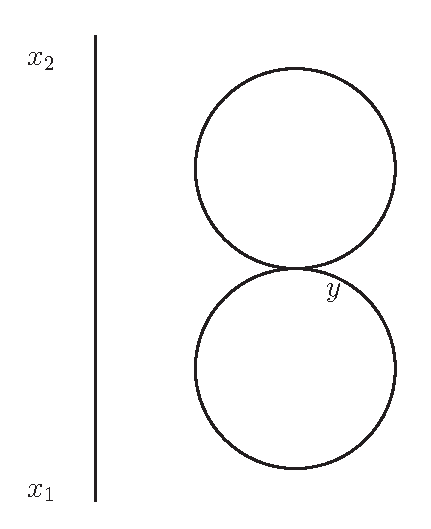
\includegraphics[width=0.4\linewidth]{QCDVertexRen/1.eps}
   &= -ig \mu^{2-d/2} (\Lambda_{(1) \, \mu}^a)_{cd} (p, q, p') \\
   \Lambda_{(1)\,\mu}^a (p, q, p') &= (t^d t^a t^d) \Lambda^{\text{QED}}_\mu (p, q, p')
\end{align*}

Evaluate the group theoretical factor
\begin{align*}
   t^d t^a t^d &= t^d \comm{t^a}{t^d} + t^d t^d t^a, \\
               &= if^{adc} t^d t^c + C_2 (F) t^a, \\
               &= -\frac{1}{2} f^{adc} f^{dcn}t^b + C_2(F)t^a, \\
               &= \left(-\frac{1}{2} C_2(G) + C_2(F) \right)t^a.
\end{align*}

Therefore
\begin{align}
   \Lambda_{(1)\,\mu}^a = \frac{g^2}{8 \pi^2 \epsilon} \left[ - \frac{1}{2} C_2 (G) + C_2 (F) \right] \gamma_\mu t^a
\end{align}

\begin{align*}
   &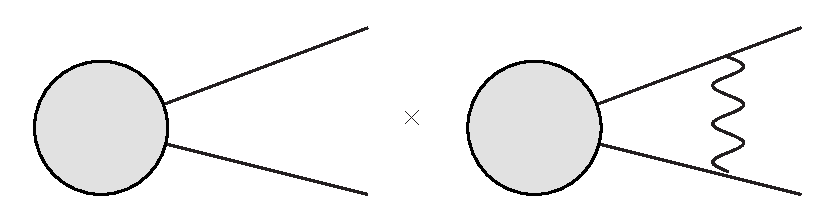
\includegraphics[width=0.5\linewidth]{QCDVertexRen/2.eps} \\
   &= -ig \mu^{2-d/2} \Lambda_{(2)\,\mu}^a \\
   &= (+ig)^2 (-g) (\mu^{4-d})^{3/2} \int \frac{\dd[d]{k}}{(2\pi)^d} \gamma^\nu (t^f)_{cd} \frac{-i}{(k-p)^2} f^{afe}  \\
   &\quad \times \left[ (p-k-q)_\nu g_{\mu\lambda} + (2k - p - p')_\mu g_{\nu\lambda} + (p' - k - q)_\lambda g_{\nu\mu} \right]\frac{-i}{(p' - k)^2} \frac{i}{\slashed{k}-m} \gamma^\lambda (t^e)_{db}\\
   \Lambda_{(2)\, \mu}^a &= \frac{g^2 \mu^{4-d}}{(2\pi)^d} f^{ade} t^f t^e I_\mu
\end{align*}

Group factor
\begin{align*}
   f^{ade} t^f t^e = \frac{i}{2} f^{afe}f^{fed}t^d = \frac{i}{2} C_2(G) t^a 
\end{align*}
Loop integral divergent part
\begin{align*}
   I_\mu = - \frac{6 \pi^2 i }{\epsilon} \gamma_\mu
\end{align*}

Thus
\begin{align}
   \Lambda_{(2)\,\mu}^a = \frac{g^2}{8 \pi^2 \epsilon} \frac{3}{2} C_2 (G) \gamma_\mu t^a
\end{align}

Combined vertex renormalization
\begin{align}
   \Lambda_{(1)\,\mu}^a + \Lambda_{(2)\,\mu}^a = \frac{g^2}{8\pi^2 \epsilon} \left[ C_2 (G) + C_2 (F) \right]\gamma_\mu t^a
\end{align}

Read off vertex renormalization $Z_{1F}$ as in QED
\begin{align}
   Z_{1F} = 1 - \frac{g^2}{8\pi^2 \epsilon} \left[ C_2 (G) + C_2 (F) \right]
\end{align}

Fermion, gauge boson self energies and fermion-gauge-boson vertex are the types of corrections that we also had in QED. Here there are more diagrams, thus other renormalization factors.
\paragraph{3-gauge-boson vertex}
\begin{align*}
   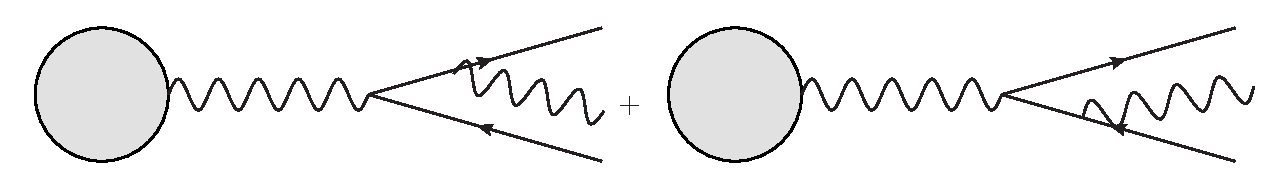
\includegraphics[width=0.9\linewidth]{QCDVertexRen/3.eps}
\end{align*}
We can show that logarithmically divergent only. Therefore only need one single subtraction, multiplicatively renormalizable!

\paragraph{4-gauge-boson vertex}
\begin{align*}
   \feynmandiagram[inline=(v.base), layered layout]{
      i1 --[gluon] v[blob] --[gluon] f1,
      i2 --[gluon] v --[gluon] f2,
   }; 
   =
   (Z_4^{-1} - 1) 
   \feynmandiagram[inline=(v.base), layered layout]{
      i1 --[gluon] v --[gluon] f1,
      i2 --[gluon] v --[gluon] f2,
   };  + \text{finite}
\end{align*}
These are also log-divergent!

\paragraph{Ghost self energy}
\begin{align*}
   \feynmandiagram[horizontal=i1 to v1, layered layout, baseline=(v1.base)]{
      i1 --[ghost] v1 [blob] -- [ghost] f1;
   };
   =  
   \feynmandiagram[horizontal=v1 to v2, layered layout, baseline=(v1.base)]{
      i1 --[ghost] v1 --[ghost] v2 -- [ghost] f1;
      v1 -- [half left, gluon] v2;
   }; 
\end{align*}
It leads to wave function renormalization $\tilde{Z}_3$.

\paragraph{Ghost-gauge vertex}
\begin{align*}
    \feynmandiagram[horizontal=i1 to v1, layered layout, inline=(v1.base)]{
      i1 --[ghost] v1 [blob] -- [ghost] f1;
      {[same layer]i2 --[gluon] v1};
   };
   = \dots = (\tilde{Z}_1^{-1} - 1)
    \feynmandiagram[horizontal=i1 to v1, layered layout, inline=(v1.base)]{
      i1 --[ghost] v1  -- [ghost] f1;
      {[same layer]i2 --[gluon] v1};
   }; + \text{finite}
\end{align*}
Renormalization factors 
\begin{align*}
   Z_1 , Z_2, Z_3, Z_4, Z_{1F}, \tilde{Z}_1, \tilde{Z}_3
\end{align*}
and $\delta_m$ for fermions.

On tree level, all couplings are inter-related. $3$-gauge, gauge-ghost and gauge-fermion all $\sim g_0$ and $4 $-gauge $\sim g_0^2$. It is consequence of gauge symmetry. If gauge symmetry unbroken by renormalization, then we expect such relations for renormalization couplings too!
Relation between various renormalization factors, analogous to $Z_1=Z_2$ in QED. "Slavnov-Taylor identities": non-abelian generalization of Ward identities in abelian theories. It can be shown using BRST transformations.

Multiply $g_0$ with $Z^{-1}$ of the corresponding vertex and with $\sqrt{Z}$ for each external leg
\begin{align*}
   \feynmandiagram[layered layout, baseline=(v.base)]{
      i1 --[gluon] v --[gluon] i2,
      i3 --[gluon] v
   };
      &\sim Z_3^{3/2} g_0 = Z_1 g \\
   \feynmandiagram[layered layout, baseline=(v.base)]{
      i1 --[gluon] v --[gluon] i2,
      i3 --[gluon] v --[gluon] i4
   };
   &\sim Z_3^2 g_0^2 = Z_4 g^2 \\
   \feynmandiagram[layered layout, baseline=(v.base)]{
      i1 -- v -- i2,
      i3 --[gluon] v
   };
      &\sim Z_2 \sqrt{Z_3} g_0 = Z_{1F} g \\
   \feynmandiagram[layered layout, baseline=(v.base)]{
      i1 --[ghost] v --[ghost] i2,
      i3 --[gluon] v
   };
      &\sim \tilde{Z}_3 \sqrt{Z_3} g_0 = \tilde{Z}_{1} g
\end{align*}
with all $g$ equal! Slavnov-Taylor identities guarantee this to hold. 

\begin{align}
   \frac{g}{g_0} &= Z_1^{-1} Z_3^{3/2} = Z_4^{-1/2} Z_3 = Z^{-1}_{1F} Z_2 Z_3^{1/2} = \tilde{Z}_1^{-1} \tilde{Z}_3 Z_3^{1/2} \notag \\
   \frac{Z_1}{Z_3} &= \frac{Z_4}{Z_1} = \frac{Z_{1F}}{Z_2} = \frac{\tilde{Z}_1}{\tilde{Z}_3}
\end{align}
This is generalization of the relation $Z_1 = Z_2$ in QED.

\section{Running Coupling}
In the chapter on the renormalization group, we learnt that from coupling constant, renormalization $g_0 \mapsto g$ and scale independence of  $g_0$, one can derive a scale dependence of the renormalized couling $g = \tilde{g}(Q^2)$. This can be characterized by the $\beta$-function,
\begin{align}
   \beta (g) = \mu \pdv{g}{\mu}
\end{align}
In perturbation theory, $\beta(g) = \beta_0 g^3 + \text{two-loops}$.

Derived solution of RG equation 
\begin{align}
   \bar{g}^2 (Q^2) = \frac{g^2}{1-\beta_0 g^2 \ln(Q^2 / \mu^2)}
\end{align}

To derive the $\beta$-function for abelian and non-abelian gauge theory. 
\paragraph{QED} the connection between bare and renormalized coupling is
\begin{align}
   e_0 &= Z_3^{-1/2} \mu^{\epsilon / 2} e, \quad  Z_3 = 1- \frac{e^2}{6\pi^2 \epsilon} \notag \\
       &= e \mu^{\epsilon/2} \left(1+ \frac{e^2}{12\pi^2 \epsilon} \right)
\end{align}

\begin{align*}
   \mu \pdv{e_0}{\mu} = 0 &= \mu^{\epsilon/2} \left[ \beta \left(1 + \frac{e^2}{12 \pi^2 \epsilon} \right) + e \frac{\epsilon}{2} \left(1+ \frac{e^2}{12\pi^2 \epsilon} \right) + \beta \frac{e^2}{6 \pi^2 \epsilon} \right] \\
   \beta(e) &= \frac{e \epsilon}{2} + \frac{e^3}{12 \pi^2} + \order{e^5} \\
   \beta(e) &\stackrel{\epsilon \rightarrow 0}{=} \frac{e^3}{12\pi^2} + \order{e^5}
\end{align*}

\paragraph{Non-abelian case}
\begin{align*}
   g_0 &= Z_{1F} Z_2^{-1} Z_3^{-1/2} \mu^{\epsilon/2} g
   \shortintertext{where}
   Z_{1F} &= 1 - \frac{g^2}{8\pi^2 \epsilon} \left[ C_2 (G) + C_2 (F) \right] \\
   Z_2 &= 1 - \frac{g^2}{8\pi^2 \epsilon} C_2 (F) \\ 
   Z_3 &= 1+ \frac{g^2}{8\pi^2 \epsilon} \left[ \frac{5}{3} C_2 (G) - \frac{2}{3} n_F \right]  \\
   g_0 &= g \mu^{\epsilon /2} \left\{ 1  + \frac{g^2}{16 \pi^2 \epsilon} \left[ -\frac{11}{3} C_2(G)  + \frac{2}{3} n_F \right] \right\}
\end{align*}
where $C_2 (G) = N$ for $\SU(N)$.

From the analogous calculation to the QED one above, we find
\begin{align}
   \beta(g) = \frac{g^3}{16 \pi^2} \left[ - \frac{11}{3} C_2(G) + \frac{2}{3} n_F \right] + \order{g^5}.
\end{align}
For $\SU(N)$ gauge theories, if $n_F < \frac{11}{2} N$, then $\beta_0 < 0$ and from the RG equation, we can conclude 
\begin{itemize}
   \item 
      asymptotic freedom $\bar{g}^2 (Q^2 \rightarrow \infty) \rightarrow 0$,
   \item infrared slavery, $\bar{g}^2$ grows for small $Q^2$, perturbation theory breaks down.
\end{itemize}

\paragraph{QCD} is $\SU(3)_\text{C}$ gauge theory of the strong interactions. Gauge bosons are called gluons, fermions are quarks. As far as we know, $n_F = 6$. So QCD shows asymptotic freedom and confinement.

Define 
\begin{align}
   \frac{1}{g^2} + \beta_0 \ln(\mu^2) &= \beta_0 \ln(\Lambda_\text{QCD}^2) \notag \\
   \alpha_s(Q^2) &= \frac{\bar{g}^2 (Q^2)}{4\pi} \notag \\
   \alpha_s (Q^2) &= \frac{12 \pi}{(33 - 2 n_F) \ln (Q^2 / \Lambda_\text{QCD}^2 )}
\end{align}
Dimensional transmutation is a mechanism to trade dimensionless $\alpha_s (\bar{g})$ with dimensionful $\Lambda_\text{QCD}$. Experimentally $\Lambda_\text{QCD} \approx \SI{200}{\mega \eV}$.

To two loops in $\overline{\text{MS}}$
\begin{align}
   \beta (g) &= \beta_0 g^3 + \beta_1 g^5 + \order{g^7} \\
   \beta_0 &= - \frac{1}{16\pi^2} \left[ \frac{11}{3} N - \frac{2}{3} n_F \right] \\
   \beta_1 &= - \frac{1}{(16\pi^2)^2} \left[ \frac{34}{3} N^2 - \left( \frac{13}{3} N - \frac{1}{N} \right) n_F\right]
\end{align}
for $N=3, n_F=6$, both terms are negative.

$n_F$ increase, then quarks screen the colour charge while gluons and ghosts lead to anti-screening. If there are too many quarks in theory, these could dominate and spoil asymptotic freedom.
